%%%%%%%%%%%%%%%%%%%%%%%%%%%%%%%%%%%%%%%%%
% Beamer Presentation
% LaTeX Template
% Version 1.0 (10/11/12)
%
% This template has been downloaded from:
% http://www.LaTeXTemplates.com
%
% License:
% CC BY-NC-SA 3.0 (http://creativecommons.org/licenses/by-nc-sa/3.0/)
%
%%%%%%%%%%%%%%%%%%%%%%%%%%%%%%%%%%%%%%%%%

%----------------------------------------------------------------------------------------
%	PACKAGES AND THEMES
%----------------------------------------------------------------------------------------

\documentclass{beamer}
\usepackage[latin1]{inputenc}
\usepackage{multirow}
\usepackage{amsmath}


\usepackage{graphicx}
\usepackage{amsmath}
\usepackage{enumerate}
\usepackage{xcolor}
\usepackage{pgfplots}
\usepackage{tikz}
\usepackage{listings}
\usepackage[linesnumbered]{algorithm2e}

\definecolor{bblue}{HTML}{4F81BD}
\definecolor{rred}{HTML}{C0504D}
\definecolor{ggreen}{HTML}{9BBB59}
\definecolor{ppurple}{HTML}{9F4C7C}

\mode<presentation> {

% The Beamer class comes with a number of default slide themes
% which change the colors and layouts of slides. Below this is a list
% of all the themes, uncomment each in turn to see what they look like.

%\usetheme{default}
%\usetheme{AnnArbor}
%\usetheme{Antibes}
%\usetheme{Bergen}
%\usetheme{Berkeley}
%\usetheme{Berlin}
%\usetheme{Boadilla}
%\usetheme{CambridgeUS}
%\usetheme{Copenhagen}
%\usetheme{Darmstadt}
%\usetheme{Dresden}
%\usetheme{Frankfurt}
%\usetheme{Goettingen}
%\usetheme{Hannover}
%\usetheme{Ilmenau}
%\usetheme{JuanLesPins}
%\usetheme{Luebeck}
\usetheme{Madrid}
%\usetheme{Malmoe}
%\usetheme{Marburg}
%\usetheme{Montpellier}
%\usetheme{PaloAlto}
%\usetheme{Pittsburgh}
%\usetheme{Rochester}
%\usetheme{Singapore}
%\usetheme{Szeged}
%\usetheme{Warsaw}

% As well as themes, the Beamer class has a number of color themes
% for any slide theme. Uncomment each of these in turn to see how it
% changes the colors of your current slide theme.

%\usecolortheme{albatross}
%\usecolortheme{beaver}
%\usecolortheme{beetle}
%\usecolortheme{crane}
%\usecolortheme{dolphin}
%\usecolortheme{dove}
%\usecolortheme{fly}
%\usecolortheme{lily}
%\usecolortheme{orchid}
%\usecolortheme{rose}
%\usecolortheme{seagull}
%\usecolortheme{seahorse}
%\usecolortheme{whale}
%\usecolortheme{wolverine}

%\setbeamertemplate{footline} % To remove the footer line in all slides uncomment this line
%\setbeamertemplate{footline}[page number] % To replace the footer line in all slides with a simple slide count uncomment this line

%\setbeamertemplate{navigation symbols}{} % To remove the navigation symbols from the bottom of all slides uncomment this line
}

\usepackage{graphicx} % Allows including images
\usepackage{booktabs} % Allows the use of \toprule, \midrule and \bottomrule in tables

%----------------------------------------------------------------------------------------
%	TITLE PAGE
%----------------------------------------------------------------------------------------

\title[BUMPER]{BUMPER: A Tool for Coping with Natural Language Searches of Millions of Bugs and Fixes} % The short title appears at the bottom of every slide, the full title is only on the title page

\subtitle{https://bumper-app.com}

\author[Mathieu Nayrolles]{\underline{Mathieu Nayrolles}, Wahab Hamou-Lhadj} % Your name
\institute[Concordia] % Your institution as it will appear on the bottom of every slide, may be shorthand to save space
{
Software Behaviour Analysis (SBA) Research Lab, ECE,  Concordia, Montr\'eal, Canada
\medskip
\textit{mathieu.nayrolles@gmail.com, wahab.hamou-lhadj@concordia.ca} % Your email address
}
\date{March 15, 2016} % Date, can be changed to a custom date

\begin{document}

\begin{frame}
\titlepage % Print the title page as the first slide
\end{frame}


\begin{frame}
\frametitle{What developers do when facing an unknow bug ?}

\begin{itemize}
  \item In 2015, we surveyed:
  \begin{enumerate}
    \item \'Ecole de Technologie Sup\'erieure, Montr\'eal, Qu\'ebec, Canada
    \item Universit\'e du Qu\'ebec \`A Montr\'eal, Montr\'eal, Qu\'ebec, Canada
    \item Concordia University, Montr\'eal, Qu\'ebec, Canada
    \item Participants of 2015 the Consortium on Software Engineering and Refactoring, Toronto, Ontario, Canada.
  \end{enumerate}


  \item When facing an unknown bug, crash or exception, where do you look for informations ?
  \item When facing an unknown bug, crash or exception, what are you searching for ?

\item Surveyed 150 people and received 89 responses (59\%)
\end{itemize}

\end{frame}

\begin{frame}
\frametitle{When facing an unknown bug, crash or exception, where do you look
for informations ?}


\begin{figure}[h!]
  \centering

  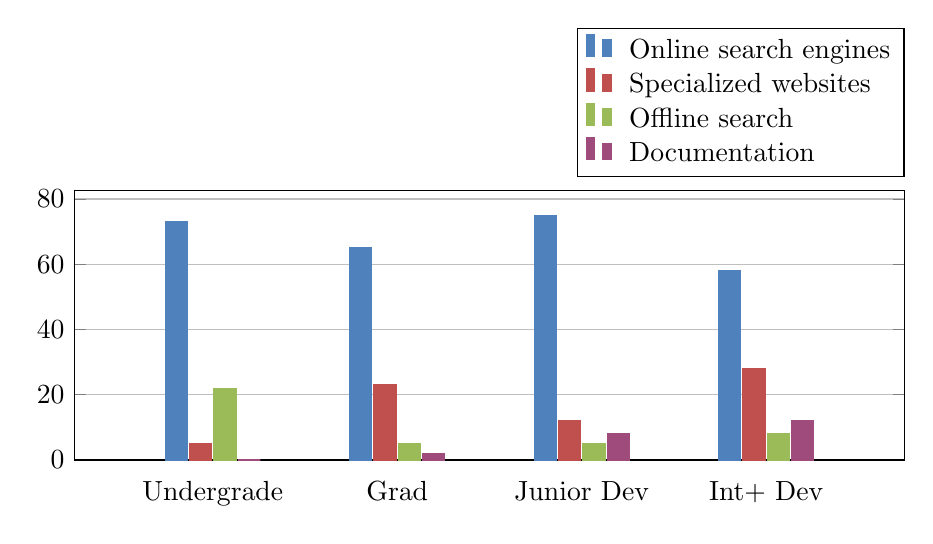
\begin{tikzpicture}
   \begin{axis}[
       width  = \textwidth,
       height = 5cm,
       major x tick style = transparent,
       ybar=2*\pgflinewidth,
       bar width=8pt,
       ymajorgrids = true,
       symbolic x coords={Undergrade, Grad, Junior Dev, Int+ Dev},
       xtick = data,
       scaled y ticks = false,
       enlarge x limits=0.25,
       ymin=0,
       legend cell align=left,
       legend style={
               at={(1,1.05)},
               anchor=south east,
               column sep=1ex
       }
   ]
       \addplot[style={bblue,fill=bblue,mark=none}]
           coordinates {(Undergrade, 73) (Grad,65) (Junior Dev,75) (Int+ Dev,58)};

       \addplot[style={rred,fill=rred,mark=none}]
             coordinates {(Undergrade, 5) (Grad,23) (Junior Dev,12) (Int+ Dev,28)};

       \addplot[style={ggreen,fill=ggreen,mark=none}]
             coordinates {(Undergrade, 22) (Grad,5) (Junior Dev,5) (Int+ Dev,8)};

       \addplot[style={ppurple,fill=ppurple,mark=none}]
           coordinates {(Undergrade, 0) (Grad,2) (Junior Dev,8) (Int+ Dev,12)};

       \legend{Online search engines, Specialized websites, Offline search , Documentation}
   \end{axis}
\end{tikzpicture}

    \caption{Answers to \textit{When facing an unknown bug, crash or exception, where do you look for informations ?} in percentage\label{fig:infos}}
\end{figure}



\end{frame}

\begin{frame}
\frametitle{When facing an unknown bug, crash or exception, what are you
searching for?}

\begin{figure}[h!]
  \centering

  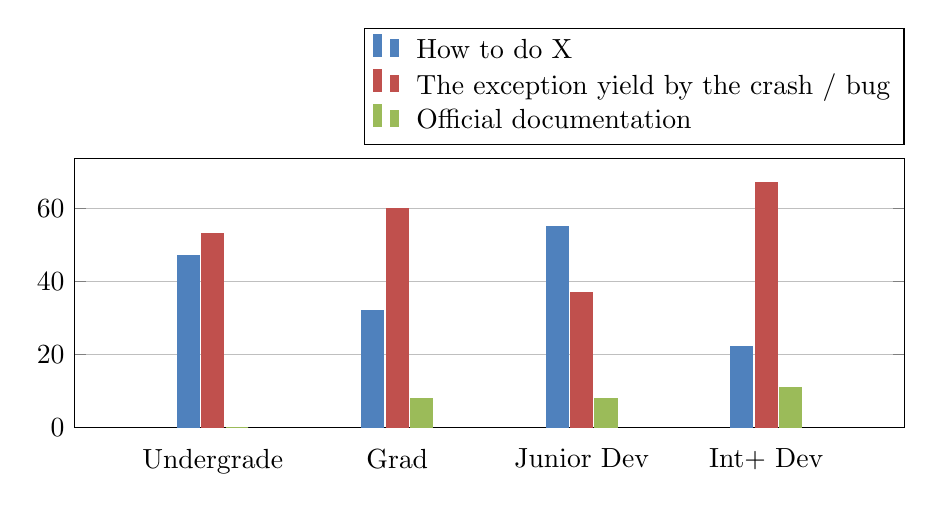
\begin{tikzpicture}
   \begin{axis}[
       width  = \textwidth,
       height = 5cm,
       major x tick style = transparent,
       ybar=2*\pgflinewidth,
       bar width=8pt,
       ymajorgrids = true,
       symbolic x coords={Undergrade, Grad, Junior Dev, Int+ Dev},
       xtick = data,
       scaled y ticks = false,
       enlarge x limits=0.25,
       ymin=0,
       legend cell align=left,
       legend style={
               at={(1,1.05)},
               anchor=south east,
               column sep=1ex
       }
   ]
       \addplot[style={bblue,fill=bblue,mark=none}]
           coordinates {(Undergrade, 47) (Grad,32) (Junior Dev,55) (Int+ Dev,22)};

       \addplot[style={rred,fill=rred,mark=none}]
             coordinates {(Undergrade, 53) (Grad,60) (Junior Dev,37) (Int+ Dev,67)};

       \addplot[style={ggreen,fill=ggreen,mark=none}]
             coordinates {(Undergrade, 0) (Grad,8) (Junior Dev,8) (Int+ Dev,11)};


       \legend{How to do X, The exception yield by the crash / bug, Official documentation}
   \end{axis}
\end{tikzpicture}
\end{figure}


\end{frame}

\begin{frame}

  \frametitle{Survey Results}

\begin{itemize}
  \item Results are not surprizing.
  \begin{enumerate}
    \item Online searches
    \item How to do X
    \item Copy/past the exception at hand
  \end{enumerate}
  \item Usually, a solution is quickly found, but ...
  \item Pain in navigating between bug report systems and code versionning systems.
\end{itemize}

\end{frame}


\begin{frame}

\frametitle{BUMPER}
\begin{itemize}
\item BUMPER: BUg Metarepository search engine for develoPErs and Researchers
\begin{itemize}
\item Aggregates information from bug report and code versionning systems
\item Online Search Engine with million bug reports AND fixes from major open-source repositories
\item Apache Software Foundation, Netbeans, Eclipse, Gnome, FireFox, Chrome, Kde, ...
\item Imports bugs reports from Bugzilla, JIRA and Github, ... and fixes from SVN, Mercurial, Git, ...
\item Natural language for developers
\item Advanced API for researchers
\end{itemize}

\end{itemize}

\end{frame}

\begin{frame}

  \frametitle{BUMPER Data (as of now)}

  \begin{table}[]
  \centering
  \begin{tabular}{c|c|c|c|c}
  \textbf{Dataset} & \textbf{R/F BR} & \textbf{CS} & \textbf{Files} & \textbf{Projects} \\ \hline \hline
  Gnome            & 550,869         & 1,231,354   & 367,245        & 512                \\ \hline
  Netbeans         & 53,258          & 122,632     & 30,595         & 39                \\ \hline
  Apache           & 49,449          & 106,366     & 38,111         & 349               \\ \hline
  Eclipse          & 78,830          & 184,900     & 21,712         & 190                \\ \hline \hline
  Total            & 732,406         & 1,645,252   & 457,663        & 1,930               \\ \hline \hline
  \end{tabular}
  \vspace{-2em}
  \end{table}

\end{frame}

\begin{frame}

  \frametitle{Google-like usage for developers}

  \begin{figure*}
    \centering
    \includegraphics[width=1\textwidth]{../media/interface.png}
  \vspace{-1.8em}
  \end{figure*}

\end{frame}

\begin{frame}

  \frametitle{Bug reports and bug fixes, side by side}

  \begin{figure*}
    \centering
    \includegraphics[width=1\textwidth]{../media/interface2.png}
  \end{figure*}

\end{frame}

\begin{frame}

  \frametitle{Using BUMPER for bug-fixing tasks}

  \textit{When I run the CSVReader with a simple main like this:}

  \noindent\begin{minipage}{0.90\linewidth}

   \lstinputlisting[language=Java, firstnumber=1, numbers=right, stepnumber=1, label=javabug, caption=Java Bug]{../media/bug.java}

  \end{minipage}

  \textit{I got the following Exception: Exception in thread ``main" java.lang.NullPointerException at CsvFileUtils.readOneLine(CsvFileUtils.java:22) at Main.main(Main.java:11). Can you please fix CsvFileUtils ?}
\end{frame}



\begin{frame}

  \frametitle{Using BUMPER for bug-fixing tasks (cont'd)}


  \begin{itemize}
    \item New survey (20 developers, 40\%  response rate)
    \item Find a suitable code snippet to fix the bug using:
    \begin{itemize}
      \item Google search engine
      \item Bumper search engine
    \end{itemize}
  \end{itemize}
  \\ \\
  \begin{itemize}
    \item Google 6.94 minutes and 7.57 web pages
    \item BUMPER 4.5 minutes and 1 web page (https://bumper-app.com)
  \end{itemize}

\end{frame}

\begin{frame}

  \frametitle{BUMPER Metamodel}

  \begin{figure*}
    \centering
    \includegraphics[width=1\textwidth]{../media/Bumper-Model.png}
  \vspace{-1.8em}
  \end{figure*}

\end{frame}

\begin{frame}

  \frametitle{API Usage for researchers}

\begin{itemize}
  \item All fields are indexed for fast search
  \item Two special indexes:
  \begin{itemize}
    \item \texttt{report\_t}: Contains a concatenation of all the bug-related fields
    \item \texttt{fix\_t}: Contains a concatenation of all the fix-related fields
  \end{itemize}
  \item Search for $"YOUR~TERMS"$ in bug reports and bug fixes:
\end{itemize}

  \begin{equation*}
  \begin{split}
  ~~(type:``BUG"~AND~report\_t:``YOUR~TERMS"\\AND~-churns:0)\\
  ~~OR~\\
  ~~(\{!parent~which=``type:BUG"\}type:~``CHANGESET"~\\AND~fix\_t:``YOUR~TERMS")
  \end{split}
  \end{equation*}

\end{frame}

\begin{frame}

  \frametitle{API usage cont'd}

\begin{itemize}
  \item Bug reports with at least one fix having:
  \begin{itemize}
    \item The word ``Exception'' in the bug report
    \item Belonging to ``Axis2'' or ``ide'' projects
    \item Reported by ``Rich'' or is ``fixed''
    \item With a ``major'' severity or a fixing time greated than 10 days
  \end{itemize}
\end{itemize}

  \begin{equation*}
  \begin{split}
    (type:``BUG"~AND~report\_t:``Exception"~\\
  ~~AND~(project:``Axis2"~OR~project:``ide")~\\
  ~~AND~(reporter:``Rich"~OR~resolution:``fixed")~\\
  ~~AND~(severity:``Major"~OR~fixing\_time:[10~TO~*])~\\
  ~~AND~-churns:0)
  \end{split}
  \end{equation*}


\end{frame}


\begin{frame}
\frametitle{Conclusion}

\begin{itemize}
\item https://bumper-app.com
\item Million bugs and associated fixes
\item Apache Software Foundation, Netbeans, Eclipse, Gnome, FireFox, Chrome, Kde, ...
\item Imports bugs from Bugzilla, JIRA  ... and fixes from SVN, Mercurial, Git, ...
\item Natural Language Search for developers
\item Advanced API for researchers
\end{itemize}



\end{frame}

%------------------------------------------------


%------------------------------------------------

\begin{frame}
\Huge{\centerline{QUESTIONS?}}
\end{frame}

%----------------------------------------------------------------------------------------

\end{document}
